\documentclass[9pt]{beamer}

\usepackage{amssymb,amsmath,mathtext}
\usepackage{indentfirst,amsfonts}
\usepackage{makecell,multirow,longtable}
\usepackage{graphicx}
\usepackage{color}
\usepackage{verbatim}


\graphicspath{{graphs/}}

\usepackage[english,russian]{babel}
\usepackage[T2A]{fontenc}
\usepackage[utf8]{inputenc}

\setbeamertemplate{navigation symbols}{}

\usetheme{Boadilla}

\beamersetuncovermixins{\opaqueness<1>{30}}{\opaqueness<2->{25}}

\setbeamerfont{frametitle}{series=\bfseries}
\setbeamerfont{block title}{series=\bfseries}

\begin{document}
\title{Нейросетевой синтез текстур с трендами}
\author{Будакян Я.\,С. \\ Научный руководитель к.т.н., доц. Грачев Е.\,А.}
\date{2017 г.} 

\maketitle

\begin{frame}\frametitle{Введение}
	Задача состоит в синтезе изображений среды, которые будут содержать в себе тренд, т.е. изменение некоторой статистической характеристики. Такими трендами могут быть, например, изменение интенсивности появления частиц среды вдоль изображения, или изменение пористости среды. \\
	\begin{figure}
		\centering{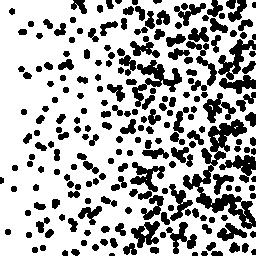
\includegraphics[width=0.35\linewidth]{trend-sample}}
		\caption{Пример текстуры с трендом интенсивности частиц}
	\end{figure}
\end{frame}

\begin{frame}\frametitle{Математическая постановка}
	С математической точки зрения, задача сводится к синтезу случайного изображения $X'$ (и построению соотвествующей процедуры синтеза), имеющего распределение, близкое к желаемому:
	$$ P_{X'} \approx P_X,$$
	где $P_X$ - распределение изображений с трендами, удовлетворяющих следующим ограничениям (для упрощения задачи):
	\begin{itemize}
		\item Это монохромные изображения 256 x 256 пикселей
		\item Изменяющимся свойством является интенсивность появления частиц $\lambda$
		\item Тренд является линейным и направлен вдоль оси x: 
		$ \lambda = \lambda_0 + kx $
	\end{itemize}
\end{frame}

\begin{frame}\frametitle{Подходы к решению задачи}
	Существует несколько подходов к решению задач подобного рода:
	\begin{itemize}
		\item 'Классический' статистический подход
		\item Первый нейросетевой подход
		\item Генеративные состязательные сети (GAN)
	\end{itemize}
\end{frame}

\begin{frame}\frametitle{'Классический' статистический подход}
	\begin{itemize}
		\item Вводится параметризированное семество распределений вероятности $P_{\theta}(x)$
		\item Параметры $\theta$ находятся из обучающей выборки:
		$$ \mathcal{L}_{\theta}(D) = \prod_{x \in D} P_{\theta}(x) $$
		$$ \theta^{*} = \underset{\theta}{\arg\max} \mathcal{L}_{\theta}(D)$$
		\item Сгенерировать семпл из $ P_{\theta^{*}}$
	\end{itemize}
	Этот подход сталкивается с проблемами:
	\begin{itemize}
		\item Пространство параметров $\theta$ может быть огромной размерности
		\item Или же известной параметрической модели распределения может вообще не существовать
	\end{itemize}
	Простой пример - генерирование человеческих лиц, похожих на реальные: параметрической модели для такой задачи не существует.
\end{frame}

\begin{frame}\frametitle{Первый нейросетевой подход}
	\begin{itemize}
		\item Вводится параметризированное семество распределений вероятности $P_{\theta}(x)$
		\begin{itemize}
			\item Вводятся скрытые переменные $V$ и функция(нейросеть) для получения $x$ из $V$ (фактически, классификация, развернутая в другую сторону)
		\end{itemize}
		\item Определяются параметры распределения (т.е. обучение нейросети)
		\item Генерируются семплы из $ P_{\theta^{*}}$
	\end{itemize}
	Этот подход возможен, однако на практике трудноосуществим.
\end{frame}

\begin{frame}\frametitle{GAN}
	Изначальная задача: найти процеруду генерирования $X'$ так, чтобы $ P_{X'} \approx P_X$.
	Переформулируем:
	$$ \rho(P_{X'}, P_X) \longrightarrow \underset{P_{X'}}{\min} $$
	\begin{itemize}
		\item Введем некоторые скрытые переменные с фиксированным распределением, например
		$$ V \sim U^n [-1, 1] $$
		\item и параметризированную процедуру генерации:
		$$ X' = g_{\theta}(V) $$
	\end{itemize}
	Переформулируем:
	$$ \rho(P_{X'}, P_X) \longrightarrow \underset{P_{X'}}{\min} $$
	$$ \rho(g_{\theta}(V), P_X) \longrightarrow \underset{g_{\theta}(V)}{\min} $$
	$$ \rho(g_{\theta}(V), P_X) \longrightarrow \underset{\theta}{\min} $$
\end{frame}

\begin{frame}\frametitle{GAN}
	Остается вопрос: что использовать в качестве метрики похожести двух распределений $\rho$, где одно из распределений задано обучающей выборкой.
	\begin{itemize}
		\item В качестве метрики статистической похожести можно использовать обученный классификатор:
		$$ \rho(P_{X'}, P_X) \longrightarrow \min \Leftrightarrow \mathcal{L} \longrightarrow \max, $$
		где $\mathcal{L}$ - функция потерь обученного классификатора.
	\end{itemize}
\end{frame}

\begin{frame}\frametitle{GAN}
	\begin{itemize}
		\item Введем две нейросети:
	\end{itemize}
\end{frame}

\begin{frame}\frametitle{Критерий качества}
\end{frame}

\begin{frame}\frametitle{Результаты, графики}
\end{frame}

\begin{frame}\frametitle{Графики-2}
\end{frame}

\begin{frame}\frametitle{Выводы}
\end{frame}

\end{document}